%%%%%%%%%%%%%%%%%%%%%%%%%%%%%%%%%%%%%%%%%
% Journal Article
% LaTeX Template
% Version 1.3 (9/9/13)
%
% This template has been downloaded from:
% http://www.LaTeXTemplates.com
%
% Original author:
% Frits Wenneker (http://www.howtotex.com)
%
% License:
% CC BY-NC-SA 3.0 (http://creativecommons.org/licenses/by-nc-sa/3.0/)
%
%%%%%%%%%%%%%%%%%%%%%%%%%%%%%%%%%%%%%%%%%

%----------------------------------------------------------------------------------------
%	PACKAGES AND OTHER DOCUMENT CONFIGURATIONS
%----------------------------------------------------------------------------------------

\documentclass[twoside]{article}

\usepackage{amssymb}
\usepackage[polish]{babel}
\usepackage{polski}

\usepackage{lipsum} % Package to generate dummy text throughout this template

\usepackage[sc]{mathpazo} % Use the Palatino font
\usepackage[T1]{fontenc} % Use 8-bit encoding that has 256 glyphs
\usepackage[utf8]{inputenc}
\selectlanguage{polish}

\linespread{1.05} % Line spacing - Palatino needs more space between lines
\usepackage{microtype} % Slightly tweak font spacing for aesthetics

\usepackage[hmarginratio=1:1,top=32mm,columnsep=20pt]{geometry} % Document margins
%\usepackage{multicol} % Used for the two-column layout of the document
\usepackage[hang, small,labelfont=bf,up,textfont=it,up]{caption} % Custom captions under/above floats in tables or figures
\usepackage{booktabs} % Horizontal rules in tables
%\usepackage{float} % Required for tables and figures in the multi-column environment - they need to be placed in specific locations with the [H] (e.g. \begin{table}[H])
\usepackage{hyperref} % For hyperlinks in the PDF

%\usepackage{lettrine} % The lettrine is the first enlarged letter at the beginning of the text
%\usepackage{paralist} % Used for the compactitem environment which makes bullet points with less space between them

\usepackage{abstract} % Allows abstract customization
\renewcommand{\abstractnamefont}{\normalfont\bfseries} % Set the "Abstract" text to bold
\renewcommand{\abstracttextfont}{\normalfont\small\itshape} % Set the abstract itself to small italic text

\usepackage{titlesec} % Allows customization of titles
%\renewcommand\thesection{\Roman{section}} % Roman numerals for the sections
%\renewcommand\thesubsection{\Roman{subsection}} % Roman numerals for subsections
\titleformat{\section}[block]{\large\scshape\centering}{\thesection.}{1em}{} % Change the look of the section titles
\titleformat{\subsection}[block]{\large}{\thesubsection.}{1em}{} % Change the look of the section titles

\usepackage{graphicx} % Required for including images
\graphicspath{{Grafika/}} % Set the default folder for images

\usepackage{fancyhdr} % Headers and footers
\pagestyle{fancy} % All pages have headers and footers
\fancyhead{} % Blank out the default header
\fancyfoot{} % Blank out the default footer
\fancyhead[C]{AGH $\bullet$ WSS i SCADA $\bullet$ Ciszewski, Dudek, Mucha $\bullet$ 2016 r.} % Custom header text
\fancyfoot[RO,LE]{\thepage} % Custom footer text

\usepackage[nottoc,numbib]{tocbibind}
\usepackage{adjustbox} %MINE: handles rotated images (like the screenshots of GUIs)
\usepackage{titletoc} %MINE: adding spacing in table of contents

%\titlecontents{section}[1.5em]
%{}
%{\contentslabel{2em}}%change the argument to obtain thedesired spacing
%{\hspace*{-2.3em}}
%{\titlerule*[1pc]{.}\contentspage}

%----------------------------------------------------------------------------------------
%	TITLE SECTION
%----------------------------------------------------------------------------------------

\title{\vspace{-15mm}\fontsize{24pt}{10pt}\selectfont\textbf{Wizualizacja danych eksperymentalnych w symulowanym środowisku linii pomiarowej w synchrotronie}} % Article title

\author{
\large
\textsc{Michał Ciszewski, Łukasz Dudek, Krystian Mucha}\\[3mm] % Your name
\textsc{Na przedmiot: Wielopoziomowe struktury sterowania i systemy SCADA}\\[3mm] % Your email address
\normalsize Prowadzący: prof. dr hab inż. Witold Bryski, mgr. inż. Andrzej Latocha\\[9mm]
\textsc{Akademia Górniczo - Hutnicza w Krakowie} % Your institution
}
\date{10 stycznia 2016 r.}

%----------------------------------------------------------------------------------------

\begin{document}
	
\begin{figure}
	\centering
	
\includegraphics[width=0.9\linewidth]{Grafika/agh_logo}
	\label{fig:agh-logo}
\end{figure}

\maketitle % Insert title

\thispagestyle{fancy} % All pages have headers and footers

\clearpage


%----------------------------------------------------------------------------------------
%	ABSTRACT
%----------------------------------------------------------------------------------------
\vspace{10mm}
\begin{abstract}

\noindent Niniejszy raport podsumowuje prace nad projektem na przedmiot ,,Wielopoziomowe struktury sterowania i systemy SCADA'' na Akademii Górniczo - Hutniczej im. S. Staszica w Krakowie. Dotyczy przygotowania dwóch sposobów wizualizacji sterowania zespołami silników w symulowanym środowisku linii badawczej w synchrotronie - aplikacji eksperckiej i klienckiej. Zostały omówione podstawy teoretyczne, środowisko programowo - sprzętowe i jego konfiguracja oraz sama realizacja projektu. W ostatnim rozdziale znajduje się instrukcja użytkowania przygotowanych aplikacji.

\end{abstract}

\smallskip
\noindent \textbf{Słowa kluczowe:} SCADA, zespoły silników, Tango Controls, Sardana, Taurus.

\tableofcontents

%----------------------------------------------------------------------------------------
%	ARTICLE CONTENTS
%----------------------------------------------------------------------------------------

\clearpage
\section{Podstawa teoretyczna}
\label{sec:podstawa}


\begin{enumerate}
	\item \textbf{Synchrotron}
	
	\hspace{2em} Synchrotron to urządzenie służące do nadawania cząstkom elementarnym (elektronom, protonom) bardzo wysokich energii za pomocą odpowiedniego układu zmiennych zsynchronizowanych pól elektrycznych i magnetycznych. W układzie tym pole elektryczne przyspieszając cząstkę przekazuje jej energię, a pole magnetyczne służy do utrzymania ruchu cząstki na torze stacjonarnym. 
	Synchrotron jest rodzajem akceleratora cząstek, w którym pole elektromagnetyczne zakrzywiające trajektorię wiązki cząstek jest synchronizowane z tą wiązką aby zwiększyć jej energię kinetyczną. W przeciwieństwie do innego rodzaju akceleratorów pole elektromagnetyczne nie jest stałe - zarówno siła jak i częstotliwość mogą się zmieniać w czasie. Pozwala to na uzyskanie ruchu po okręgu o stałym promieniu przez cały czas trwania procesu przyspieszania cząstek. Schemat synchrotronu przedstawiono na rys. (\ref{fig:schematSynchrotronu}).
	
	\begin{figure}[ht]
		\centering
		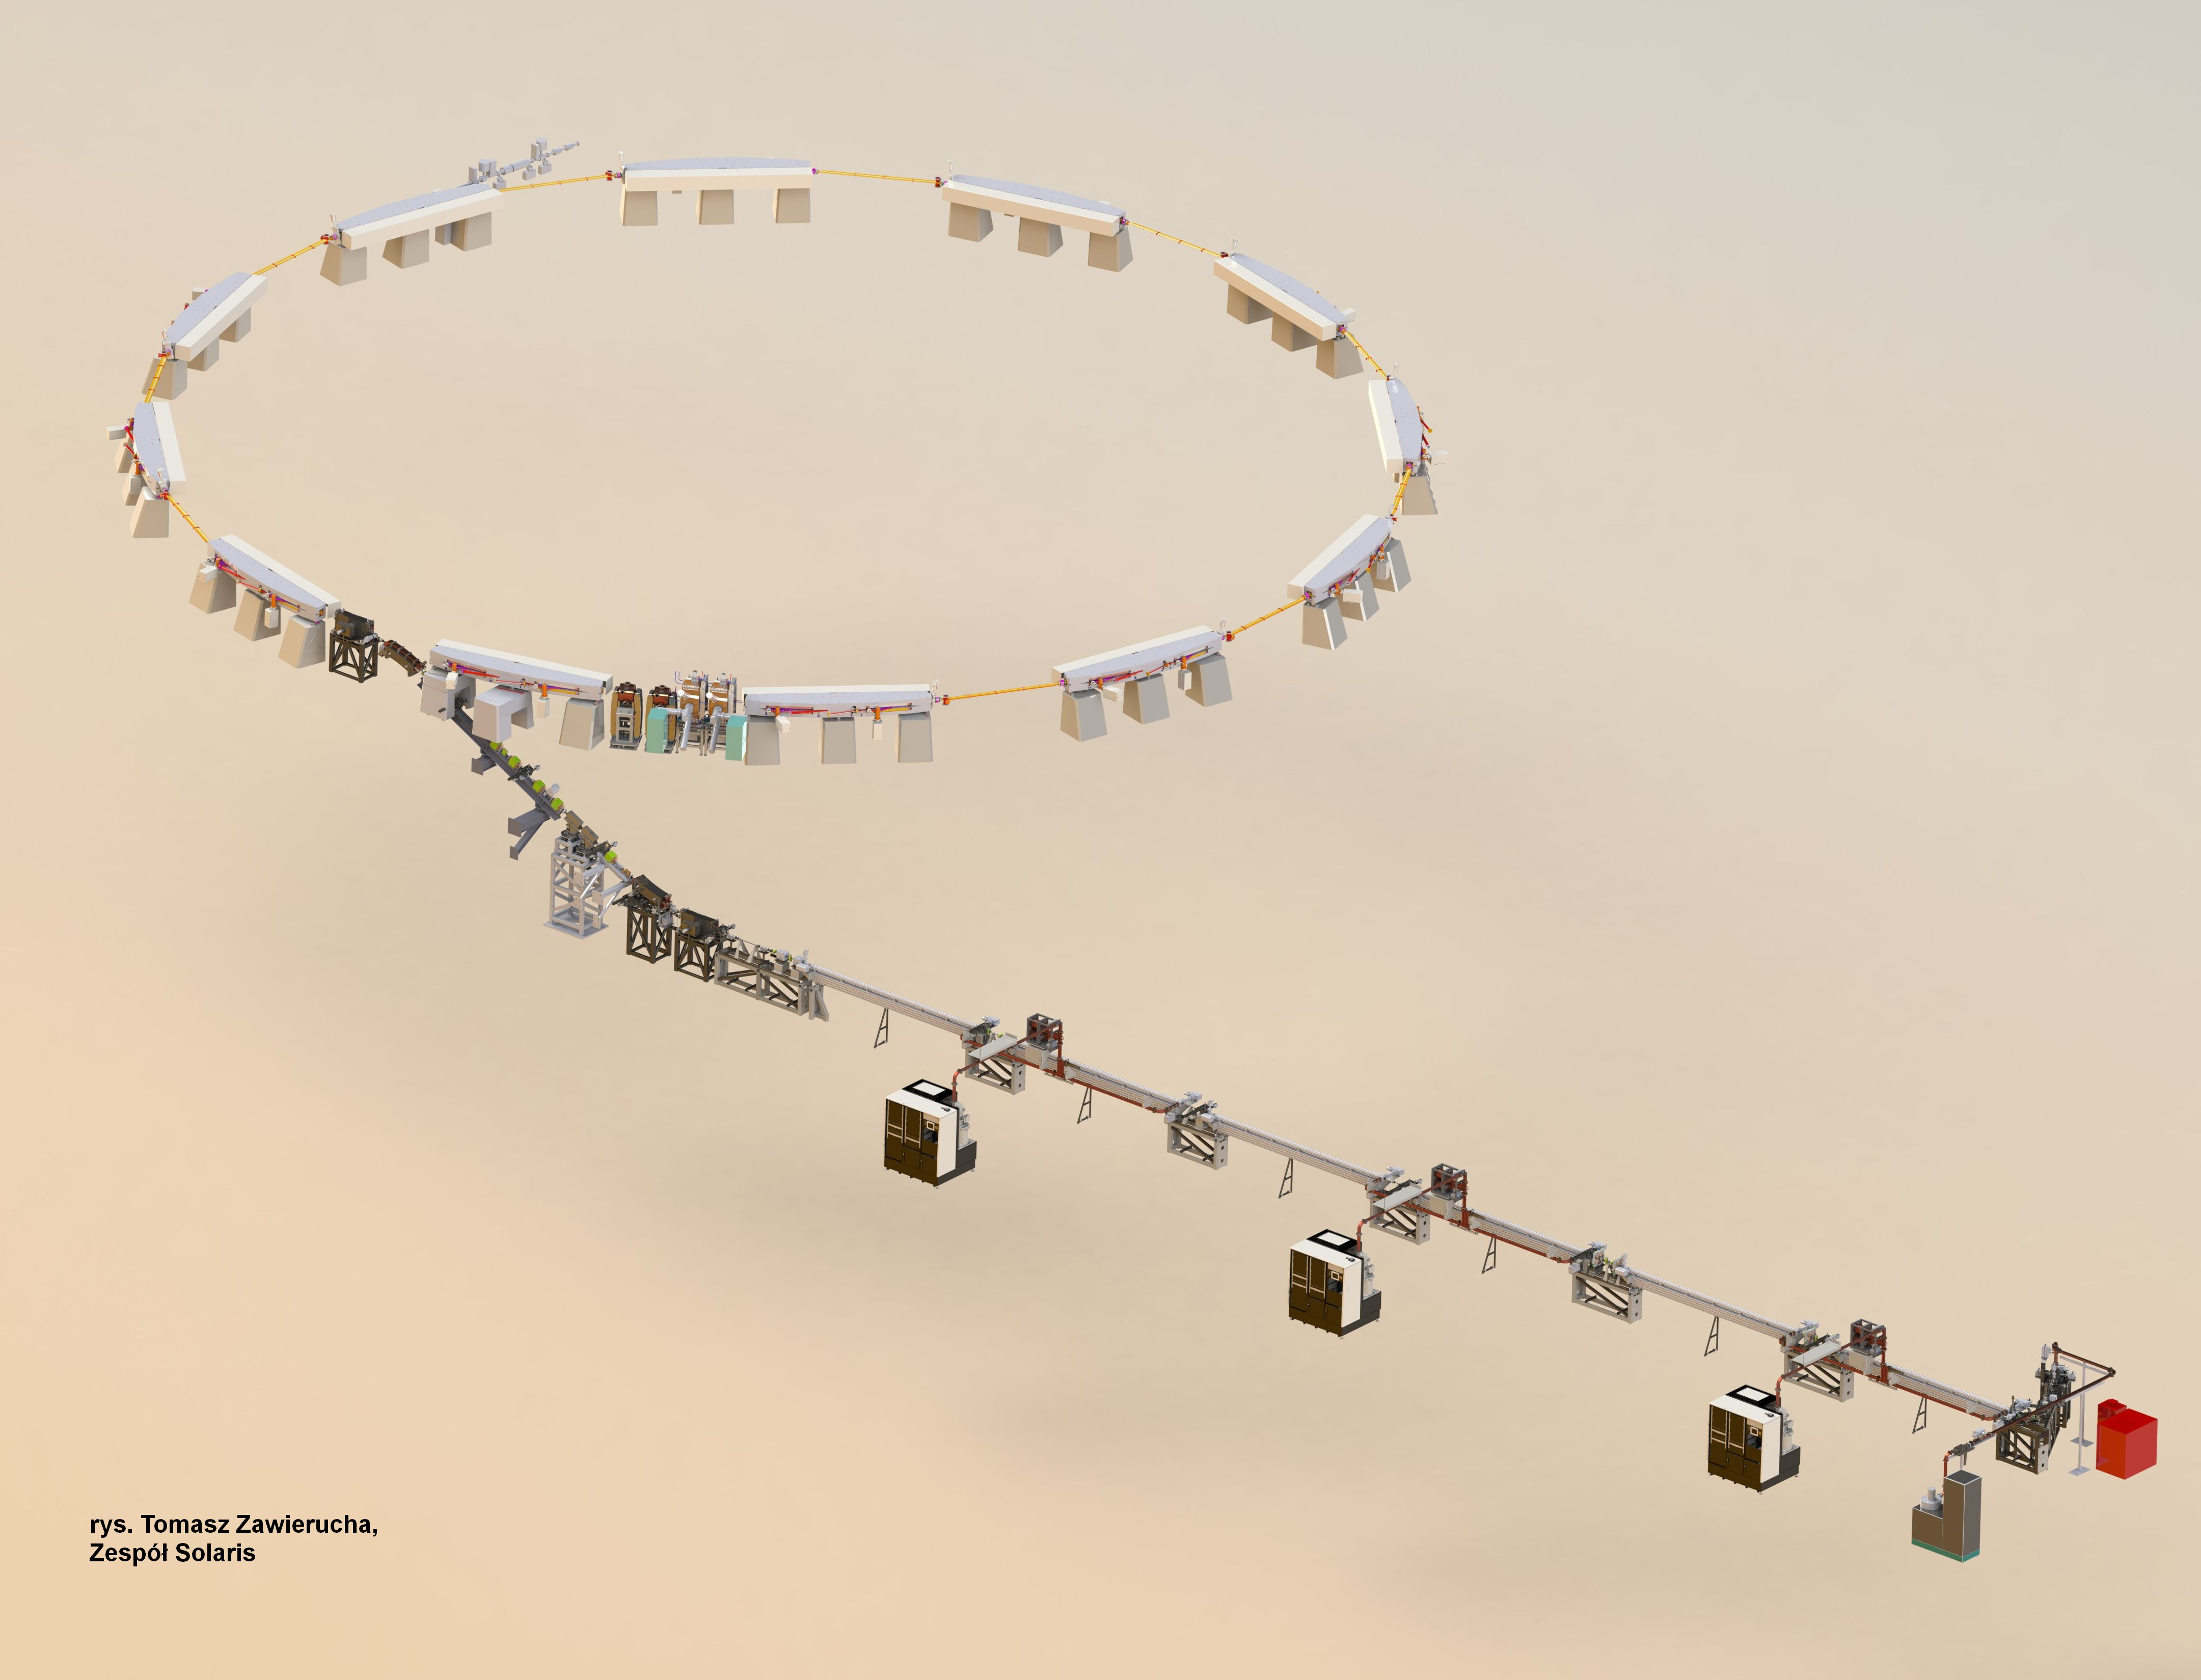
\includegraphics[width=0.9\linewidth]{Grafika/solarisMaszyna}
		\caption{Schemat synchrotronu znajdującego się w Solarisie. Źródło: \cite{synchrotron_uj_edu}}
		\label{fig:schematSynchrotronu}
	\end{figure}
	
	
	\hspace{2em} Promieniowanie synchrotronowe, jakie emituje pierścień akumulacyjny badane jest w specjalnych liniach badawczych, w skład których wchodzą skomplikowane mechanizmy składajace się z różnego rodzaju przesłon, zwierciadeł, pryzmatów itp. Każdy z tych elementów sterowany jest silnikiem krokowym, stąd istnieje konieczność synchronicznej pracy tych silników. Schemat lini badawczej przestawiono na rys. (\ref{fig:schematliniBadawczej})
	\newline
	\newline
	\newline
	
	\begin{figure}[ht]
		\centering
		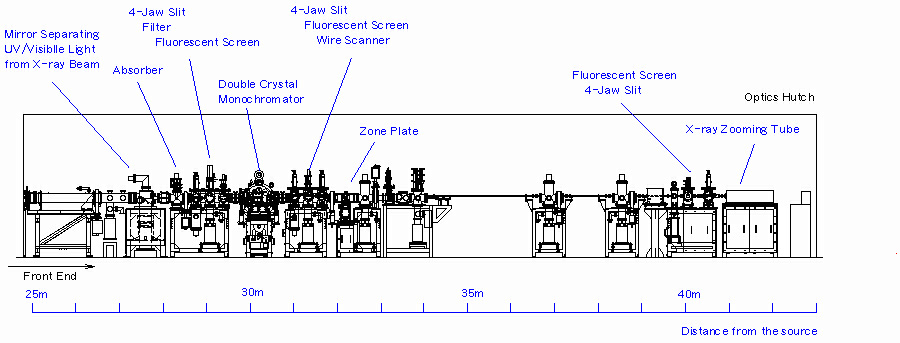
\includegraphics[width=0.9\linewidth]{Grafika/liniaBadawcza}
		\caption{Schemat lini badawczej.}
		\label{fig:schematliniBadawczej}
	\end{figure}
	
	\item \textbf{Systemy SCADA}
	
	\hspace{2em}Systemy SCADA (ang. Supervisory control and data acquisition) to system do zdalnego monitorowania i sterowania procesem techologicznym. Głównymi funkcjami systemów SCADA są:
	
	\begin{itemize}
		\item zbieranie aktualnych danych (pomiarów)
		\item wizualizacja danych
		\item sterowanie procesem
		\item alarmowanie
		\item archiwizacja danych	
	\end{itemize}
	
	\hspace{2em}Systemy te dają możliwość współpracy ze sterownikami PLC, regulatorami mikroprocesorowymi i innymi urządzeniami. Pozwalają na realizację zdecentralizowanych systemów automatyki przemysłowej. Systemy SCADA pozwalają na uzyskanie szybkiego wglądu w faktyczny stan urządzeń produkcyjnych i wykonawczych. Są one doskonałym sposobem nie tylko na zamianę języka maszyn na język ludzi, ale także umożliwiają szybką lokalizację alarmów, podstawowe logowanie danych czy też automatyczną reakcję na określone sygnały pochodzące z urządzeń. System SCADA w warstwie graficznej odpowiada za jednoznaczne zaprezentowanie dynamicznie zmieniającej się informacji. Jednocześnie zdefiniowane przez użytkownika algorytmy logiczne przyspieszają i wspomagają operatora w jego pracy. System SCADA jest także podstawowym źródłem danych dla systemów nadrzędnych i przemysłowych baz danych.
	
\end{enumerate}


\section{Koncepcja realizacji}


\clearpage
\section{Specyfikacja sprzętu}
\label{sec:spec_sprzet}

\quad W przypadku tak stricte programowego projektu, jak opisywany w niniejszym raporcie ciężko jest wyróżnić jakąś szczególną specyfikację potrzebnego sprzętu. Do realizacji wykorzystywaliśmy tylko komputer klasy PC z oprogramowaniem opisanym w rozdziale \ref{sec:spec_prog}.

To, o czym jednak należy tutaj wspomnieć, to używane zwykle w synchrotronach zestawy silników krokowych, które mają specyficzne możliwości konfiguracyjne oraz mogą być prosto zintegrowane z rozproszonym systemem sterowania zarządzanym przy pomocy narzędzi Tango. Najczęściej stosowanym rozwiązaniem jest platforma programowo - sprzętowa IcePAP \cite{web:icepap}.

\clearpage
\section{Specyfikacja programowo-sprzętowa}
\label{sec:spec_prog}

\subsection{Sprzęt}
\quad W przypadku tak stricte programowego projektu, jak opisywany w niniejszym raporcie ciężko jest wyróżnić jakąś szczególną specyfikację potrzebnego sprzętu. Do realizacji wykorzystywaliśmy tylko komputer klasy PC z oprogramowaniem opisanym w podrozdziale \ref{sub:plat_prog}.

To, o czym jednak należy tutaj wspomnieć, to używane zwykle w synchrotronach zestawy silników krokowych, które mają specyficzne możliwości konfiguracyjne oraz mogą być prosto zintegrowane z rozproszonym systemem sterowania zarządzanym przy pomocy narzędzi Tango. Najczęściej stosowanym rozwiązaniem jest platforma programowo - sprzętowa IcePAP \cite{web:icepap, proc:icepap}.

\subsection{Platformy programowe}
\label{sub:plat_prog}

\begin{enumerate}
	\item \textbf{Tango}
	
	\hspace{2em}System sterowania TANGO jest darmowym zestawem narzędzi do sterowania dowolnego rodzaju sprzętem lub oprogramowaniem oraz do budowy systemów SCADA (ang. Supervisory Control And Data Acquisition). Jest to oprogramowanie typu open-source wykorzystywane do sterowania synchrotronami, laserami oraz innymi eksperymentami fizycznymi. TANGO jest aktywnie rozwijane przez TANGO Consortium.
	
	\hspace{2em}TANGO jest rozproszonym systemem sterowania. Oznacza to, że może działać zarówno na jednej maszynie, jak i na wielu. Wykorzystuje dwa protokoły sieciowe - COBRA oraz Zeromq. Podstawowym modelem komunikacji jest model klient-serwer. Komunikacja pomiędzy klientem i serwerem może być synchroniczna, asynchroniczna (COBRA) oraz sterowana zdarzeniem (Zeromq) \cite{TangoWiki}.
	
	\hspace{2em}System TANGO jest opakowaniem (ang. wrapper) dla protokołu COBRA zapewniającym przyjazne dla użytkownika API. Dzięki takiemu podejsciu wiele detali związanych z nawiązywaniem i utrzymywaniem połączenia pomiędzy urządzeniami jest niewidoczna dla użytkownia, co pozwala na szybsze i łatwiejsze rozbudowywanie systemu sterowania.
	
	\hspace{2em}TANGO wykorzystuje MySQL jako bazę danych do trzymania informacji. Informacjami takimi mogą byc np. nazwy urządzeń, adresy sieciowe, listy urządzeń itp. MySQL jest relacyjną bazą danych implementującą podzbiór SQLa. System TANGO jest wspierany przez 4 platformy: Linux, Windows NT, Solaris oraz HP-UX.
	
	\begin{enumerate}
		\item \textbf{Taurus}
		
		\hspace{2em}Taurus jest platformą programistyczną dla Pythona służącą do sterowania oraz akwizycji danych w zastosowaniach naukowych oraz przemysłowych. Pozwala na szybkie i proste tworzenie interfejsów użytkownika. Jest to częśc pakietu programistycznego Sardana. Taurus posiada bogatą bibliotekę dzięki czemu stworzone GUI (ang. Graphical User Interface)  może zawierać wiele różnych komponentów takich jak wykresy, tabele, przyciski itp. Celem biblioteki Taurus jest zapewnienie przyjaznego API dla użytkownika oraz przyspieszenie procesu rozwijania aplikacji bazowanych na TANGO.
				
		
		\item \textbf{Sardana}
		
		\hspace{2em}Sardana to pakiet oprogramowania do nadzoru, kontroli i akwizycja danych w zastosowaniach naukowych. Jej celem jest zredukowanie kosztów oraz czasu potrzebnych do projektowania, rozwijania oraz utrzymywania systemów SCADA. Rozwój Sardany zapoczątkowany został przy synchrotronie ALBA, a dzisiaj jest wspierany przez wiekszą społeczność,  w skład której wchodzą liczne laboratoria oraz inne jednostki (ALBA, DESY, MaxIV, Solaris, ESRF).
		Sardana jest bazowana na systemie TANGO i wykorzystuje bibliotekę Taurus umożliwiającą programowanie i konfigurację interfejsu użytkownika \cite{Sardana}.
		
		%\item \textbf{Jive}
		\item \textbf{TangoBox9} (maszyna wirtualna)
		
		W związku z polityką udostępniania oprogramowania na otwartych licencjach, konsorcjum Tango wypuściło gotową wirtualną maszynę, która zawiera wszystkie narzędzia pakietu Tango zainstalowane na systemie Ubuntu 14.04 64-bit. Są tam uwzględnione również wszystkie poboczne projekty, które ułatwiają korzystanie z systemu i dostarczają dodatkowych opcji potrzebnych systemowi sterowania, np. archiwizacji, logowania czy tworzenia interfejsów użytkownika. W tym systemie dostarczono w pełni funkcjonalne symulacyjne środowisko systemu sterowania synchrotronem z uwzględnieniem jednej linii badawczej. Obecne są tam również podstawowe aplikacje będące częścią bazowej paczki Tango, takie jak: Astor (służy do zarządzania serwerami urządzeń), Pogo (generator kodu serwerów), Jive czy AtkMoni (umożliwiają konfigurację i testowanie samych urządzeń).
		
	\end{enumerate}
	\item \textbf{Python}
	
	\hspace{2em}Python to wysokopoziomowy język programowania ogólnego przeznaczenia. Posiada rozbudowane pakiety bibliotek standardowych. Ideą przewodnią Pythona jest czytelność i klarowność kodu źródłowego. Jego składnia cechuje się przejrzystością i zwięzłością. W Pythonie możliwe jest programowanie obiektowe, programowanie strukturalne i programowanie funkcyjne. Typy sprawdzane są dynamicznie, a do zarządzania pamięcią stosuje się garbage collection. Python rozprowadzany jest na otwartej licencji umożliwiając także zastosowanie do zamkniętych komercyjnych projektów \cite{Python}.
	
	\begin{enumerate}
		\item \textbf{PyCharm}
		
		\hspace{2em}PyCharm to zintegrowane środowisko programistyczne (IDE) dla języku programowania Python firmy JetBrains. Zapewnia m.in.: edycję i analizę kodu źródłowego, graficzny debugger, uruchamianie testów jednostkowych, integrację z systemem kontroli wersji. Wspiera także programowanie i tworzenie aplikacji internetowych w Django.
		
		\hspace{2em}Jest oprogramowaniem wieloplatformowym pracującym na platformach systemowych: Microsoft Windows, Linux oraz OS X. Wydawany jest w wersji Professional Edition, które jest oprogramowaniem zamkniętym oraz w wersji darmowej Community Edition, które pozbawione jest jednak niektórych funkcjonalności w porównaniu z wersją komercyjną \cite{PyCharm}.
		
	\end{enumerate}
	\item \textbf{QtDesigner}
	
	\hspace{2em}Jest to narzędzie slużące do projektowania graficznego interfejsu użytkownika (GUI), zawarte w wieloplatformowym środowisku programistycznym Qt Creator.
\end{enumerate}

\clearpage
\section{Opis realizacji}
\label{sec:opis_realizacji}

\quad Realizacja zadań projektowych opisanych w rozdziale \ref{sec:koncepcja} została przeprowadzona przy użyciu wszystkich technologii, które są wymienione w rozdziałach \ref{sec:spec_sprzet} i \ref{sec:spec_prog}. Można ją podzielić na trzy główne części, które zostaną przedstawione w kolejnych podrozdziałach.

\subsection{Konfiguracja wirtualnego środowiska}
\label{sub:konfiguracja}
\quad Pierwszym elementem, który należało opanować było uruchomienie wirtualnej maszyny ,,TangoBox9'', a następnie konfiguracja wszystkich elementów niezbędnych do realizacji postawionego celu. Kolejne kroki postępowania zostały przedstawione poniżej:

\begin{enumerate}
	\item Sprawdzenie funkcjonowania systemu Tango: głównej bazy danych, poszczególnych ,,serwerów urządzeń'' (ang. device servers) oraz samych urządzeń. W tym celu użyto dwóch aplikacji stanowiących pakiet do zarządzania systemem Tango: Astor i Jive. Weryfikacja poprawności polegała na uruchomieniu obu aplikacji i wizualnym sprawdzeniu stanów interesujących z punktu widzenia projektu komponentów systemu.
	\item Sprawdzenie funkcjonowania dodatków do systemu Tango: archiwizacji, bibliotek Taurus i Sardana. Należało uruchomić odpowiednie aplikacje (,,jhdbconfigurator'' w przypadku archiwizacji, ,,taurusgui'' - Taurusa i ,,Sardemo'' - Sardany) i sprawdzić, czy nie wyrzucają jakiś błędów.
	\item Uruchomienie serwerów urządzeń zarządzających silnikami. Klasa ,,Motors'' jest częścią oprogramowania ,,Pool'', które należy do pakietu Sardana. Program Astor umożliwia włączenie serwera.
	\item Konfiguracja silników. Zostały ustawione następujące elementy:
	\begin{enumerate}
		\item urządzenie ,,motor/motctrl01/1'':
		\begin{enumerate}
			\item zakres wartości położenia: -120, 120,
			\item progi alarmowe: -110, 110,
			\item progi ostrzeżeń: -100, 100,
			\item pozycje czujników krańcowych - takie, jak zakresy wartości położenia,
			\item prędkość: 10,
			\item przyspieszenie: 0,5.
		\end{enumerate}
		\item urządzenie ,,motor/motctrl01/2'':
		\begin{enumerate}
			\item zakres wartości położenia: -120, 120,
			\item progi alarmowe: -110, 110,
			\item progi ostrzeżeń: -100, 100,
			\item pozycje czujników krańcowych - takie, jak zakresy wartości położenia,
			\item prędkość: 100,
			\item przyspieszenie: 40.
		\end{enumerate}
		\item urządzenie ,,motor/motctrl01/3'':
		\begin{enumerate}
			\item zakres wartości położenia: -50, 50,
			\item progi alarmowe: -45, 45,
			\item progi ostrzeżeń: -40, 40,
			\item pozycje czujników krańcowych - takie, jak zakresy wartości położenia,
			\item prędkość: 10,
			\item przyspieszenie: 0,1.
		\end{enumerate}
		\item urządzenie ,,motor/motctrl01/4'':
		\begin{enumerate}
			\item zakres wartości położenia: -90, 140,
			\item progi alarmowe: -85, 130,
			\item progi ostrzeżeń: -80, 125,
			\item pozycje czujników krańcowych - takie, jak zakresy wartości położenia,
			\item prędkość: 100,
			\item przyspieszenie: 1.
		\end{enumerate}
	\end{enumerate}
\end{enumerate}

\subsection{Opracowanie aplikacji eksperckiej i operatorskiej}


\subsection{Testy}

\clearpage
\section{Opis załączonego kodu}
\label{sec:opis_kodu}

\quad Załączone do niniejszego raportu archiwum w formacie ZIP, stanowiące techniczno - implementacyjną część projektu stanowi zrzut repozytorium, które zostało założone na potrzeby projektu. Zawiera następujące elementy:
\begin{enumerate}
	\item Katalog ,,OperatorGUI'':
	\begin{enumerate}
		\item Plik Pythona ,,editable\_mano\_meter.py'' zawierający definicję klasy wykresów kołowych użytych w aplikacji operatora.
		\item Plik Pythona ,,operator\_gui.py'' zawierający definicję całej aplikacji operatora.
		\item Plik ,,operator\_gui.ui'' będący podstawą aplikacji operatora utworzoną przy pomocy programu QtDesigner.
	\end{enumerate}
	\item Katalog ,,Raport'' zawierający niniejszy raport oraz jego pliki źródłowe w języku LaTeX. Ten opis nie zawiera jego dokładnej zawartości, jako że nie jest on częścią kodu napisanego na potrzeby projektu.
	\item Plik Pythona ,,\_\_init\_\_.py'' potrzebny Pythonowi, aby odpowiednio rozpoznał pliki w tym języku znajdujące się wewnątrz tego katalogu.
	\item Pliki konfiguracyjne aplikacji eksperckiej: ,,config.xml'' oraz ,,config.py''.
	\item Skrypt ,,ExpertGUI'' służący do uruchomienia aplikacji eksperckiej.
	\item Plik ,,macro\_sequence\_motors\_showcase.xml'' stanowiący zapis sekwencji makr.
	\item Plik ,,motors\_positions.pck'' stanowiący zapis konfiguracji wykresu w aplikacji eksperckiej.
	\item Plik ,,README.md'' opisujący skrótowo zawartość katalogu projektowego.
	\item Plik ,,wizard.log'' zawierający podsumowanie generacji ustawień aplikacji eksperckiej.
	\item Pliki konfiguracyjne repozytorium.
\end{enumerate}

\clearpage
\section{Instrukcja użytykownika}
\label{sec:manual}

\quad Jak zostało wcześniej wspomniane, możliwość interakcji z systemem silników została przewidziana w formie dwóch aplikacji. Niniejszy rozdział został poświęcony opisowi możliwych schematów wykorzystania przygotowanego oprogramowania. Podstawą obu jest opisywana w rozdziale \ref{sec:spec_prog} biblioteka Taurus, a konkretniej jej część (o nazwie ,,TaurusGUI'') umożliwiająca programowanie bądź konfigurację głównych okien interfejsów użytkownika.

\subsection{Aplikacja ekspercka}
\label{sub:expertgui}

\quad Pierwsza z utworzonych aplikacji to interfejs ekspercki - został on przedstawiony na rysunku \ref{fig:ExpertGUI}. Umożliwia on sprawowanie pełnej kontroli nad procesem sterowania silnikami, a więc również nad przeprowadzaniem eksperymentów na linii badawczej. Została ona podzielona na 4 części oraz dwa menu:

\begin{enumerate}
	\item Część w lewym górnym rogu zawiera dwa panele. Pierwszy o nazwie ,,Macros'', widoczny na rysunku przedstawiającym aplikację ekspercką, to panel umożliwiający użytkownikowi wybór odpowiedniej, pojedynczej komendy spośród obfitego zestawu dostępnych, ustawienie jej parametrów i uruchomienie. Wybór odbywa się poprzez kliknięcie odpowiedniej pozycji na rozwijanej liście. Uruchomić makro można przyciskiem ,,Play'' - obok niego znajdują się również przyciski do wstrzymywania i przerywania działania komendy. Dioda w ostatnim wierszu pokazuje stan urządzenia, które zajmuje się wykonywaniem makr - kolory odpowiadają standardom Tango, opisanym w rozdziale \ref{sec:spec_prog}.
	
	Drugi panel - ,,Macro Description'' - zawiera opis wybranego makra. Przedstawia on skrótowy opis działania komendy oraz znaczenie i zakres wszystkich jej parametrów - zarówno wejściowych, jak i wyjściowych (jeśli dane makro cokolwiek zwraca). Znajdują się tam również czasem dodatkowe informacje lub fakty, na które warto zwrócić uwagę. Wyboru można dokonywać zarówno na poprzednim panelu w tej części aplikacji, jak i na panelu ,,Sequence'', opisanym niżej.
	
	\item Część w prawym górnym rogu zawiera aż 4 panele. Pierwszy z nich, widoczny na rysunku, to panel ,,Sequence''. Zawiera on opcje pozwalające na wykonywanie, zapisywanie i wczytywanie sekwencji makr. Pierwsza z tych operacji jest aktywowana przyciskiem ,,Play'', podobnie, jak na panelu ,,Macros'' (jak również przyciski umożliwiające wstrzymanie i przerwanie działania makra). Możliwość tworzenia nowej sekwencji, otwierania istniejącej i zapisywania bieżącej dają (w takiej właśnie kolejności) przyciski, które znajdują się w górnym lewym rogu panelu.
	
	Po wybraniu makra z rozwijanej listy można je dodać do edytowanej sekwencji przyciskiem ,,+'' znajdującym się w prawym górnym rogu panelu. Przyciski poniżej ,,+'' umożliwiają odpowiednio usunięcie makra z sekwencji, przesunięcie go w górę lub w dół na liście obrazującej kolejność wykonywania oraz zmianę poziomu wykonywania makra (dotyczy tylko niektórych, powiązanych komend). Po wybraniu makra na liście sekwencji uaktywnia się dolna lista na panelu, która zawiera konfigurację wszystkich argumentów wejściowych makra.
	
	Pozostałe panele w tej części aplikacji eksperckiej - ,,DoorOutput'', ,,DoorDebug'' oraz ,,DoorResult'' - zawierają informacje zwrotne uzyskiwane po uruchomieniu makra (bądź ich sekwencji). Znajdują się tam odpowiednio komunikaty, wiadomości dotyczące odpluskwiania makra (jeśli uruchomione jest ono w takim trybie) oraz wyniki ewentualnych obliczeń. W przygotowanej na potrzeby sekwencji makr te panele nie są wykorzystywane.
	
	\item Część znajdująca się w lewym dolnym rogu zawiera tylko jeden panel - ,,Positions''. Jest on interaktywnym wykresem, aktualizowanym na bieżąco w czasie rzeczywistym (okres oczekiwania na odświeżenie wynosi 1 do 3 sekund). Zmiennymi, których wartości przedstawia są położenia wszystkich czterech silników, stanowiących podstawę niniejszego projektu. Ten panel daje użytkownikowi bardzo dużo możliwości - większość z nich jest dostępna poprzez kliknięcie prawym przyciskiem myszy na wykres. Pokazuje się wtedy menu kontekstowe, które zawiera takie opcje, jak:
	\begin{itemize}
		\item dostosowywanie ustawień osi (wybór zakresów, zmiana trybu z liniowego na logarytmiczny, określenie kolorów odpowiadających poszczególnym sygnałom, itp.),
		\item ustawienie zmiennych prezentowanych na wykresie,
		\item zapisanie i wczytanie aktualnych ustawień wykresu,
		\item zmianę tytułu,
		\item dostosowanie skal osi (oraz opcję autoskalowania),
		\item włączanie/wyłączanie pokazywania wartości minimalnej/maksymalnej oraz legendy,
		\item obliczanie większej ilości parametrów statystycznych.
	\end{itemize}
	Dodatkowo, klikanie na nazwy atrybutów w legendzie pozwala wyłączać pokazywanie odpowiadającej im krzywej na wykresie lub przełączanie się między prawą i lewą osią Y.
	
	\item W prawym dolnym rogu aplikacji eksperckiej znajdują się dwa panele - ,,/slit'' oraz ,,/mirror''. Oba umożliwiają bezpośrednie poruszanie silnikami bądź grupami silników. Każdy z nich zawiera pola do wpisywania wartości zadanych oraz monitorowania aktualnego położenia silników. Przycisk ,,Stop'', znajdujący się między polami każdego silnika pozwala zatrzymać ruch. Po lewej stronie, zaraz za nazwą silnika, znajdują się przyciski ,,-'' oraz ,,+''. Pozwalają one na wykonanie pojedynczego kroku odpowiednim silnikiem.
	
	Kluczową sprawą dla użytkowania aplikacji jest zwracanie uwagi na format wpisywanych w polach edycyjnych danych. Normalna czcionka oznacza brak różnic między wartością zadaną a aktualnym położeniem. W takim stylu są też wyświetlane wartości po uruchomieniu aplikacji. Kolor niebieski i pogrubienie czcionki znamionują obecność takich zmian - można je zatwierdzić, używając klawisza Enter. Użytkownik może również chcieć zaaplikować wartość wyświetlaną w normalnym stylu (na czarno) - w tym celu przewidziano kombinację klawiszy Ctrl + Enter. Żółty kolor czcionki oznacza wartość, która przekroczyła poziom ostrzeżenia. Kolor żółty oraz czerwona ramka naokoło pola edytowalnego - wartość przekraczającą poziom alarmowy.
	
	\item Dodatkowymi elementami aplikacji są 2 menu oraz dioda znajdująca się w prawym dolnym rogu. Jej ciągłe miganie to efekt ,,bicia serca'' (ang. hearbeat), czyli proste sprawdzenie, czy aplikacja działa, czy się zacięła.
	
	Pierwsze menu znajduje się na samej górze aplikacji. Składa się z dwóch części - jedna to standardowe menu aplikacji, w którym znajdziemy takie opcje jak zapisanie perspektywy, zmianę widoku, opcje wyświetlania i ukrywania paneli, itp. Poniżej znajdują się przyciski menu narzędziowego - umożliwiają one szybki dostęp do maksymalizacji okna, wczytania perspektywy (czyli aktualnie wyświetlanej konfiguracji paneli) oraz dodanie nowego panelu.
	
	Drugie menu znajduje się w pasku po prawej stronie aplikacji. Obecne tam 4 ikony to odpowiednio - logo organizacji, logo aplikacji, przycisk paniki (zatrzymuje wszystkie aktualnie wykonywane operacje) oraz tryb inspekcji.
\end{enumerate}


\begin{figure}[ht]
	\begin{adjustbox}{addcode={
				\begin{minipage}{\width}}
					{\caption{Zrzut ekranu pokazujący aplikację ekspercką.}\label{fig:ExpertGUI}
				\end{minipage}},rotate=90,center}
		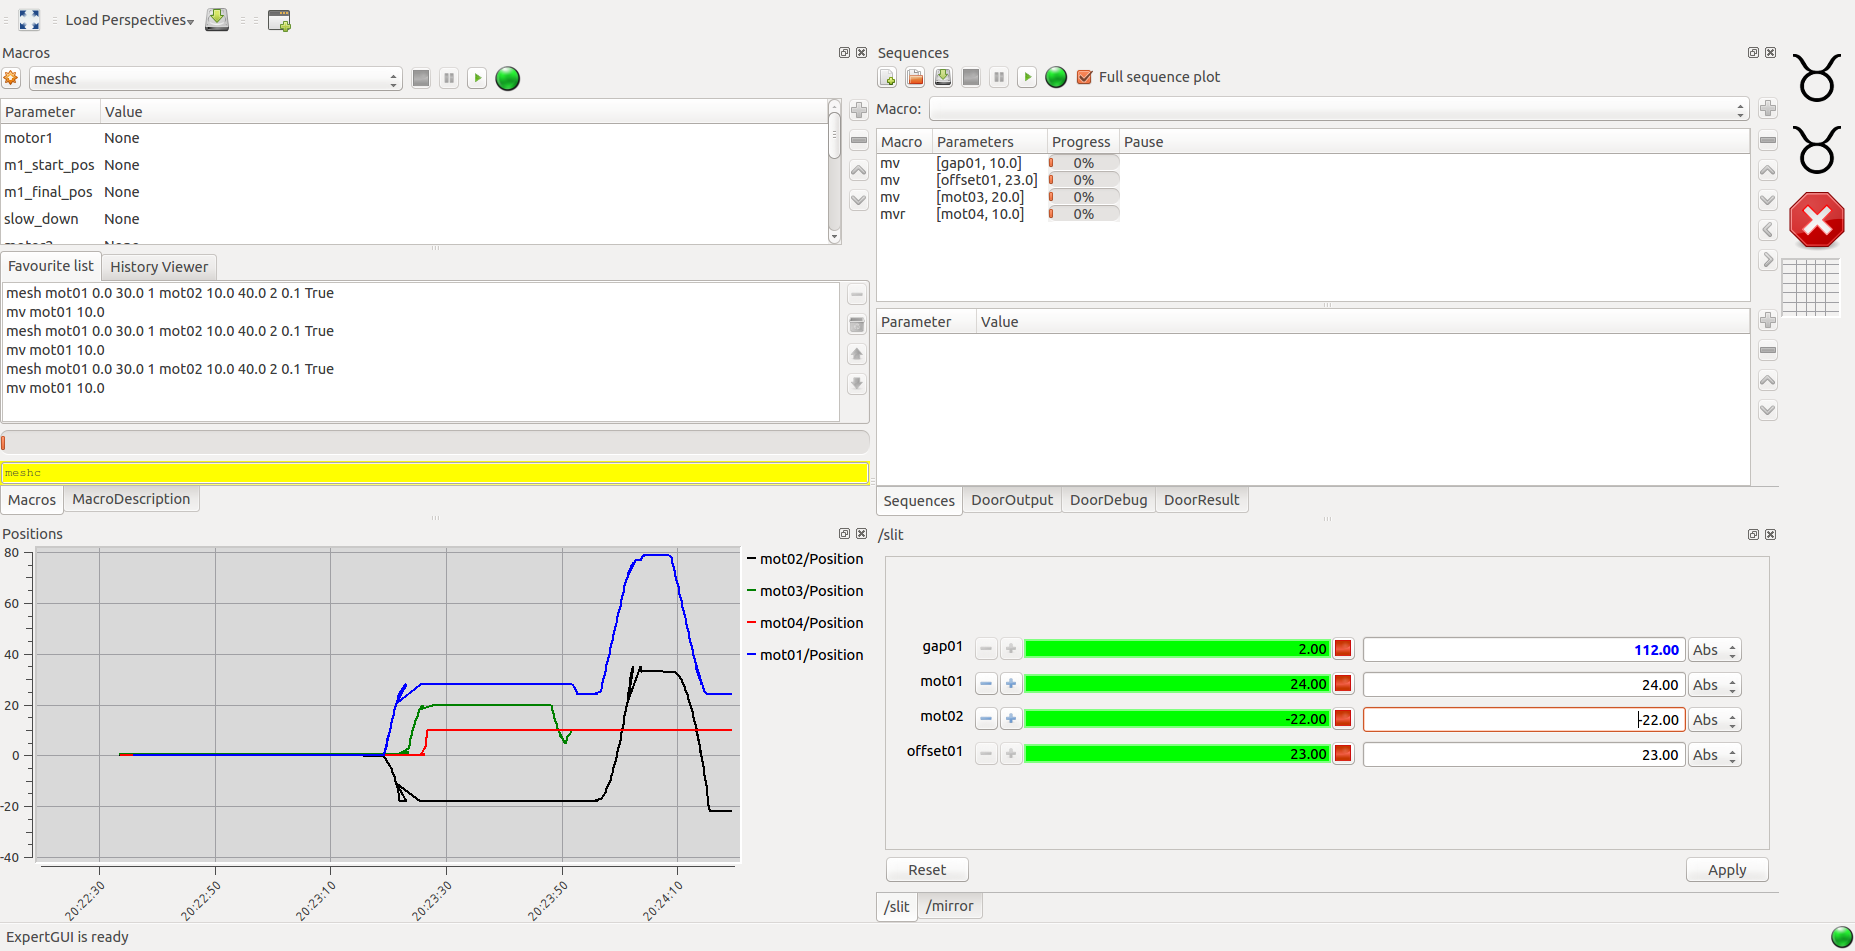
\includegraphics[scale=.32]{Grafika/ExpertGUI}
	\end{adjustbox}
\end{figure}

Przykładowe użycie aplikacji mogłoby obejmować następujące kroki:
\begin{enumerate}
	\item Uruchom aplikację poprzez wywołanie skryptu: \texttt{./ExpertGUI}.
	\item Wczytaj zapisaną perspektywę, sekwencję makr i ustawienia wykresów.
	\item Sprawdź, czy wszystko jest gotowe do przeprowadzenia eksperymentu (w szczególności należy zadbać o właściwą kolejność makr i odpowiednie dla nich argumenty).
	\item Włącz sekwencję makr.
	\item Monitoruj położenie silników na wykresie.
	\item W razie potrzeby, dopasuj ręcznie pozycję (lub zostaw to operatorowi).
\end{enumerate}


%---------------------------------------------------------------------------------------------------
\subsection{Aplikacja kliencka}
\label{sub:operatorgui}

\quad Druga z utworzonych aplikacji to interfejs klienta lub operatora - jest on przedstawiony na rysunku \ref{fig:OperatorGUI}. Pozwala on tylko na poruszanie konkretnymi silnikami w - operator może skorygować w niewielkim zakresie wartość położenia każdego elementu ruchomego i zobaczyć aktualny stan poszczególnych silników.

Ta aplikacja zawiera tylko jeden typ panelu - taki sam dla wszystkich czterech silników, którymi operator może sterować. Każdy z tych paneli zawiera następujące elementy:
\begin{enumerate}
	\item Nazwę silnika (według konwencji Tango).
	\item Diodę określającą stan urządzenia (odpowiadającą standardowej kolorystyce wykorzystywanej w Tango). Na rysunku \ref{fig:OperatorGUI} są widoczne trzy możliwe stany urządzenia związanego z silnikiem.
	\item Duże, zielone pole statusu. Jego rozmiar jest warunkowany najdłuższym możliwym komunikatem, który jest w nim wyświetlany. Jak widać na rysunku \ref{fig:OperatorGUI}, może prezentować różne rodzaje informacji statusowej.
	\item Wykres kołowy aktualizowany na bieżąco, który pokazuje pozycję silnika.
	\item Pole edytowalne służące do wpisywania pożądanej wartości zadanej położenia silnika. Podlega dokładnie takim samym regułom, jak to w aplikacji eksperckiej, opisane w podrozdziale \ref{sub:expertgui}.
\end{enumerate}

Najechanie kursorem na dowolny element powyższej listy (oprócz nazwy silnika) powoduje pokazanie się widocznej na rysunku \ref{fig:OperatorGUI} podpowiedzi dotyczącej atrybutu dołączonego do danego elementu aplikacji. W przypadku pozycji pokazują się tam takie informacje, jak zakres, poziomy ostrzeżenia i alarmu.

Aplikacja operatora, tak jak opisywane wcześniej oprogramowanie eksperta, posiada menu bazowe aplikacji opartej o TaurusGUI, a więc umożliwiające m.in. konfigurację widoku oraz tworzenie perspektyw.

Przykładowy proces korzystania z aplikacji może być przedstawiony w następujących krokach:
\begin{enumerate}
	\item Uruchom aplikację poleceniem: \texttt{python OperatoGUI/operator\_gui.py}
	\item Sprawdź, czy stany wszystkich silników umożliwiają poruszenie nimi.
	\item Dokonaj odpowiednich korekt w położeniu.
\end{enumerate}


\begin{figure}[ht]
	\begin{adjustbox}{addcode={
				\begin{minipage}{\width}}
					{\caption{Zrzut ekranu pokazujący aplikację operatora.}\label{fig:OperatorGUI}
				\end{minipage}},rotate=90,center}
				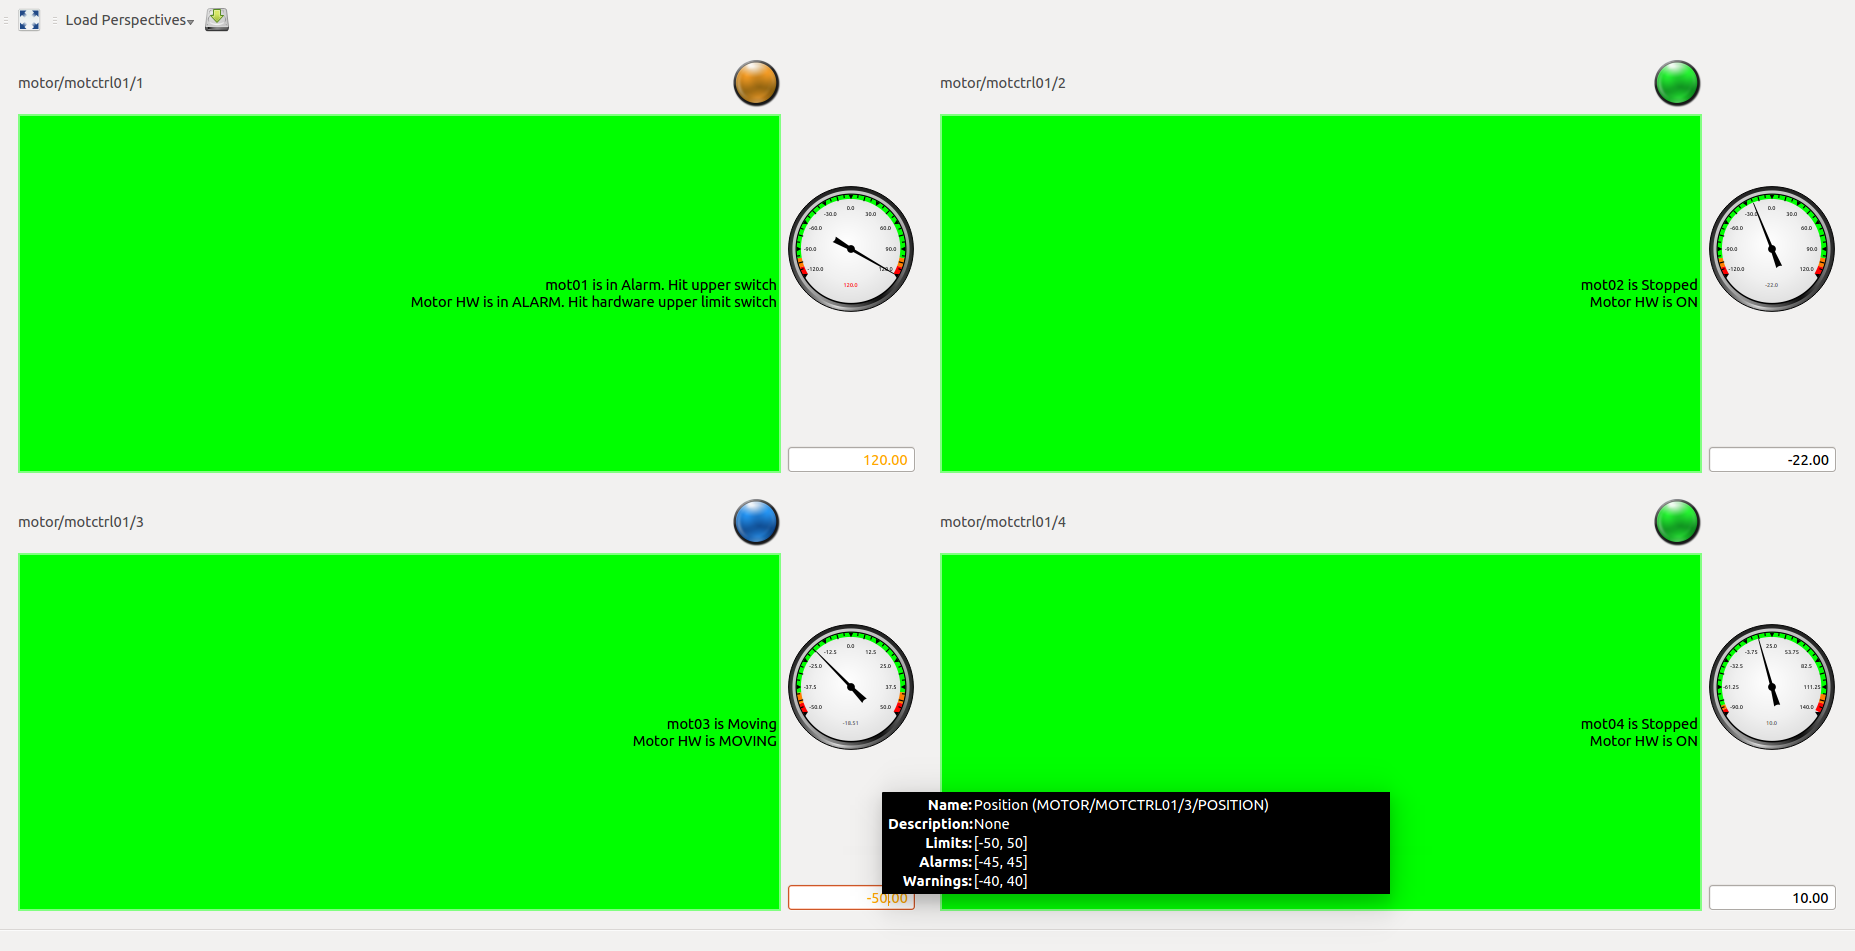
\includegraphics[scale=.32]{Grafika/OperatorGUI}
	\end{adjustbox}
\end{figure}

%----------------------------------------------------------------------------------------
%	REFERENCE LIST
%----------------------------------------------------------------------------------------

\clearpage
\bibliographystyle{alpha}
\begin{thebibliography}{99} % Bibliography - this is intentionally simple in this template

\bibitem{web:tango}
Strona internetowa Tango Controls.
\newblock \texttt{http://www.tango-controls.org/} .
\newblock Zarządzane przez: Stowarzyszenie Tango.
\newblock Stan na: 10.01.2016 r.

\bibitem{web:taurus}
Dokumentacja zestawu narzędzi Taurus.
\newblock \texttt{http://www.taurus-scada.org/en/stable/} .
\newblock Zarządzane przez: ALBA Synchrotron.
\newblock Stan na: 10.01.2016 r.

\bibitem{web:sardana}
Dokumentacja zestawu narzędzi Sardana.
\newblock \texttt{http://sardana.readthedocs.org/en/stable/} .
\newblock Zarządzane przez: ALBA Synchrotron.
\newblock Stan na: 10.01.2016 r.

\bibitem{web:icepap}
Strona internetowa poświęcona zestawowi silników IcePAP.
\newblock \texttt{http://www.esrf.eu/\\Instrumentation/DetectorsAndElectronics/icepap} .
\newblock Zarządzane przez: ESRF.
\newblock Stan na: 10.01.2016 r.

\bibitem{proc:icepap}
Janvier, N., Clement, J. M., Fajardo, P.,  
\newblock{\em IcePAP: An Advanced Motor Controller for Scientific Applications in Large User Facilities}.
\newblock W materiałach: ICALEPCS 2013, San Francisco, Kalifornia, USA.

\bibitem{TangoWiki}
System TANGO
\newblock \texttt{https://en.wikipedia.org/wiki/TANGO} .
\newblock Stan na: 13.01.2016 r.

\bibitem{Sardana}
Sardana Home Page
\newblock \texttt{http://www.sardana-controls.org/en/stable/} .
\newblock Stan na: 13.01.2016 r.

%\bibitem{GMeansExplanation}
%Użytkownik 'ashenfad'.
%\newblock{\em Divining the 'K' in K-means Clustering}.
%\newblock \texttt{http://blog.bigml.com/2015\\/02/24/divining-the-k-in-k-means-clustering/}. 
%\newblock Dodane: 24.02.2015 r.
%\newblock Stan na: 05.12. 2015 r.


\end{thebibliography}

\end{document}
